\documentclass[svgnames]{beamer}
%\usepackage[usenames,dvipsnames,svgnames,table]{xcolor}
% \mode<presentation>{\usetheme{Ilmenau}} % Ilmenau
% \mode<presentation>{\usetheme{Warsaw}} % Warsaw
\mode<presentation>{\usetheme{Darmstadt}} % Darmstadt
% behaviors

% toc before each section
% \AtBeginSection[]
% {
% \begin{frame}{Table of Contents}
% \tableofcontents[currentsection]
% \end{frame}
% }

% \AtBeginSection{\frame{\sectionpage}}
% \AtBeginSubsection{\frame{\subsectionpage}}
% \AtBeginSubsubsection{\frame{\subsubsectionpage}}

% add number of page
\beamertemplatenavigationsymbolsempty
\setbeamerfont{page number in head/foot}{}
\setbeamertemplate{footline}[frame number]

% add number of page
% \addtobeamertemplate{navigation symbols}{}{%
%     \usebeamerfont{footline}%
%     \usebeamercolor[fg]{footline}%
%     \hspace{1em}%
%     \insertframenumber/\inserttotalframenumber
% }

% remove symbols
\setbeamertemplate{navigation symbols}{}

% headers
\title{CSRF attack: even Google was vulnerable.}
\author{Quentin Lemaire \& David Kufa}
\date{\today}

% content
\begin{document}
  
\maketitle % build title

% Hello,
% This presentation will be about:
% ...

% introduction
\section*{Introduction}
\begin{frame}
\frametitle{Introduction}
\begin{itemize}
  \item \textit{Cross-Site Request Forgery} (CSRF) also known as ``sea surf''
  \item Mix of theoretical \& practical explanations about CSRF.
  \item Presentation of 2 Google stories related to CSRF
\end{itemize}

\end{frame}

% toc

% CSRF:
% - What is it ? How it works ? How to identify it ?
% - How to exploit it ? How to prevent it ?
% Google stories:
% - Description
% (- Exploitation) really fast
% - Impact (different !)
\begin{frame}
  \frametitle{Summary}
  \tableofcontents
\end{frame}

%% ------- %%

\section{CSRF}
% \begin{frame}
%   \frametitle{CSRF}
%   \tableofcontents[currentsection]
% \end{frame}

% description
\subsection{What is it ?}
\begin{frame}
  \frametitle{What is CSRF ?}
  % TODO text description
  \begin{itemize}
   \item Web vulnerability discovered in 2001
   \item Top 8 from OWASP\footnote{\textit{Open Web Application 
       Security Project}: \url{https://www.owasp.org/}} most critical 
   web application security risks in 2013
   \item Uses victims' lack of knowledge \& websites vulnerability
  \end{itemize}
  
  \pause
  
  \begin{block}{Idea of the attack}
    Forging fake HTTP(S) requests in order to execute legitimate actions on the user's behalf.
  \end{block}

  
%C. Shiflett said (compared to XSS) : "Cross-Site Request Forgeries are an almost opposite style of attack. Rather than exploiting the trust that a user has for a website, they (CSRF attacks) exploit the trust that a website has for a user"


% alertblock
% exampleblock
%   \begin{block}{CSRF}
%     Sea surf uiuiui
%   \end{block}
\end{frame}

\subsection{How it works ?}
\begin{frame}
  \frametitle{Concrete scenario}
  \begin{figure}[h!t]
  \begin{center}
    \fbox{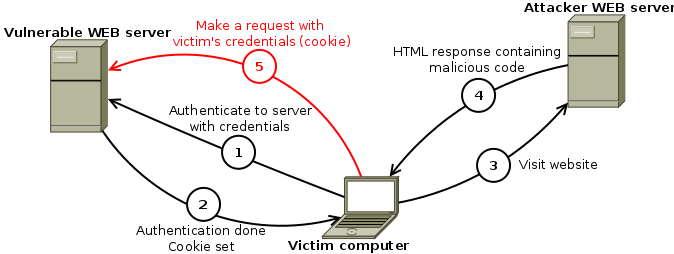
\includegraphics[width=\textwidth]{media/CSRF_attack.png}}
    \caption{
      CSRF attack scenario. Diagram realized with Dia (\url{https://wiki.gnome.org/Apps/Dia/}).
    }
  \end{center}
  \end{figure}
\end{frame}

\subsection{How to prevent it ?}
% exploitation & prevention
\begin{frame}
  \frametitle{Exploitation \& prevention} % say we built the webapp from scratch
  % TODO insert video(s)
\end{frame}


%% ------- %%


\section{Google was vulnerable}
\begin{frame}
  \frametitle{Google was vulnerable}
  \tableofcontents[currentsection]
\end{frame}

\subsection{Story 1}

\begin{frame}
  \frametitle{Description}
\end{frame}

\begin{frame}
  \frametitle{Exploitation}
\end{frame}

\begin{frame}
  \frametitle{Impact}
\end{frame}


\subsection{Story 2}

\begin{frame}
  \frametitle{Description}
\end{frame}

\begin{frame}
  \frametitle{Exploitation}
\end{frame}

\begin{frame}
  \frametitle{Impact}
\end{frame}

\section*{Conclusion}
\begin{frame}
  \frametitle{Best practices}
  \begin{itemize}
   \item Users
   \pause
   \begin{itemize}
    \item Disconnect from websites
    \item Be careful when you click on URL % received by email most of the time
    \item Use several browsers (or extension to disable JavaScript\footnote{NoScript for instance: \url{https://noscript.net/}})
   \end{itemize}
   \pause
   \item Developers
   \begin{itemize}
    \item Methods presented previously: tokens, referer, CAPTCHA, etc.
    \pause
    \item \textcolor{ForestGreen}{Use robust \textbf{frameworks}!}
   \end{itemize}

  \end{itemize}
\end{frame}


\begin{frame}
  \frametitle{Thanks}
  \begin{center}
    Thank you very much for your attention!
  \end{center}
\end{frame}


\end{document}